\chapter{Реализация имитатора абонентов сети Modbus}
В данном разделе приводится описание реализации программы имитатора абонентов сети Modbus
с использованием языка программирования \cpp и библиотеки~\texttt{Qt}
на основе результатов, полученных в главах~\ref{sec:part1} и \ref{sec:part2}.


\section{Определение Modbus тегов} \label{sec:modbus_tag}
Не смотря на то что в самом протоколе Modbus передаются только целые числа, некоторые производители Modbus устройств,
в том числе производители средств разработки для программируемых логических контроллеров, расширяют возможности протокола
для передачи вещественных чисел одинарной и двойной точности, так и целочисленных значений размером до восьми байт \cite{book:gost:modbus_program_language}.
Принимая во внимание эти данные и результаты из главы \ref{sec:part2},
становится возможным определить программную реализацию типов данных.
Каждый тег является программной реализацией метакласса \mbelement из раздела \ref{sec:ontology_modbus}
и описывается тремя обязательными и двумя необязательными атрибутами,
отражающими свойства из таблицы \ref{tbl:modbus_data_properties}.
К обязательным относятся:
\begin{itemize}
    \item[\texttt{title}] заголовок тега, относящийся к предметной области;
    \item[\texttt{address}] адрес тега, согласованный с адресным пространством контроллера;
    \item[\texttt{type}] тип передаваемого значения, который может принимать следующие значения, в зависимости от группы:
    %
    \begin{itemize}
        \item[BOOL] 1 бит;
        \item[WORD] 16 бит;
        \item[DOUBLEWORD] 32 бита;
        \item[REAL] 32 бита;
        \item[LONGREAL] 64 бита.
    \end{itemize}
\end{itemize}
Необязательные атрибуты служат для вспомогательной цели:
\begin{itemize}
    \item[\texttt{position}] первично -- определяет положение сигнального проводника на модуле в сборке контроллера;
    вторично -- обозначает, что это результат промежуточных вычислений контроллера;
    \item[\texttt{description}] описание передаваемого параметра.
\end{itemize}

Теги объединены в конфигурационный файл, пример которого показан 
в листинге \ref{lst:modbus_tags_example} в приложения \ref{app:sec:modbus_tag}.
В файле содержится совокупность тегов (\textit{индивидов}),
% каждый из которых представляет \textit{объект} --- экземпляр класса \mbelement,
с набором необходимых атрибутов: обозначение, назначение, положение, адрес, тип данных, значение.
На конфигурационный файл для тегов накладываются условия,
как показано в листинге \ref{lst:modbus_tags_example_configs} приложения \ref{app:sec:xsd}.


\section{Ненормализованная таксономия классов}\label{sec:writers_relationship}

На основе анализа предметной области строится ненормализованная\footnote{любой класс может иметь два и более не пересекающихся надкласса}
иерархия классов для управления информационной моделью,
диаграмма взаимосвязи классов представлена на рисунке \ref{fig:modbus_class_uml} \cite[стр. 223]{book:oop:oop_analize}.
\begin{landscape}\begin{figure}[h!]\begin{center}
    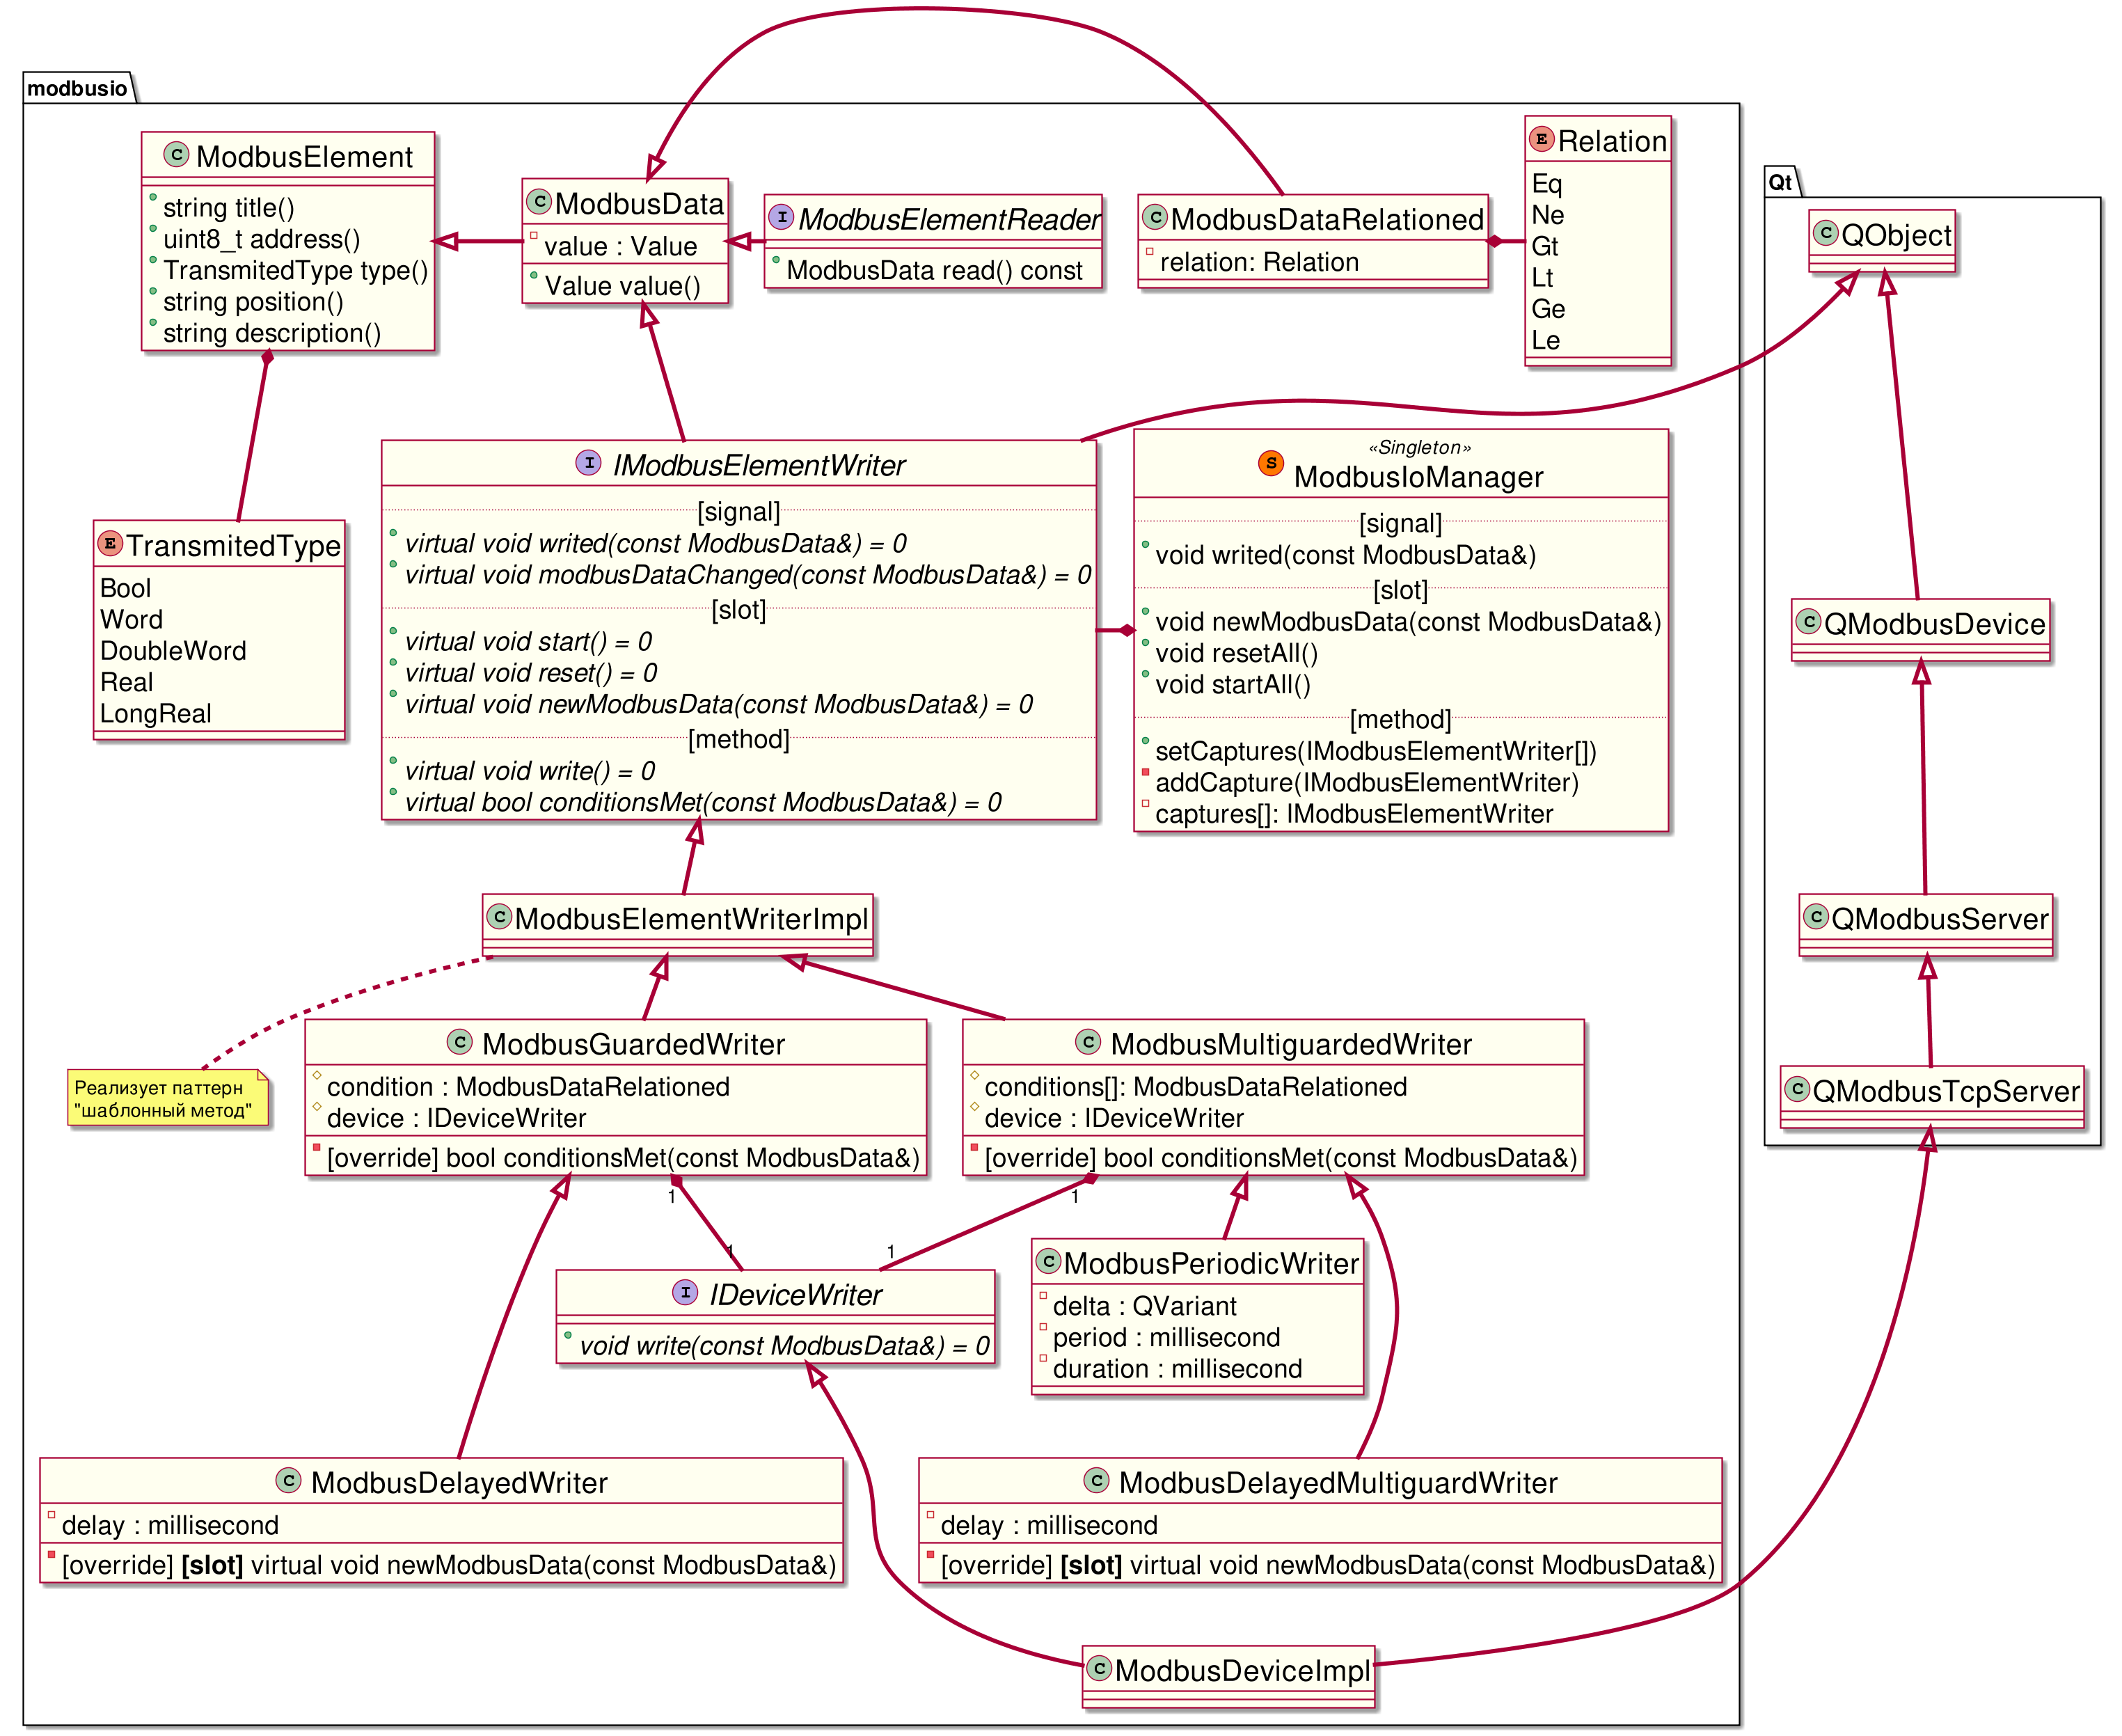
\includegraphics[height=.88\textheight,keepaspectratio]{modbus_class_relationship.png}
    \caption[Иерархия классов имитатора]
        {UML диаграмма классов имитатора модели АНПА при передачи по шине данных типа Modbus.}
            \label{fig:modbus_class_uml}
\end{center}\end{figure}\end{landscape}

Базовый класс \mbelement инкапсулирует в себе представление тега из раздела \ref{sec:modbus_tag}.
Для передачи данных между компонентами системы используется класс \mbdata, производный от \mbelement,
в котором появляется дополнительный член класса \texttt{value} для хранения политипных значений
(то есть для хранения типа \texttt{xsd:aniURI} возможно использовать тип \texttt{std::variant} начиная с \cppseventeen
или его аналог \texttt{QVariant} из библиотеки \texttt{Qt}).
Для реализации поведения используется полиморфизм, так как классы имеют один и тот же протокол \cite[стр. 133]{book:oop:oop_analize}.

Интерфейс \mbreader введен для общности, но в данной работе представляет мало интереса.

\subsection{Жизненный цикл компонента \texttt{IModbusElementWriter}}
Отметим, что этот компонент создается с использованием множественного наследования:
первый супер-класс это \mbdata, инкапсулирующий передаваемые данные,
а второй --- \texttt{QObject}, так как необходимо получить <<ортогональные свойства>>
(механизм сигналов-слотов и обработка сообщений) \cite[стр. 134]{book:oop:oop_analize},
для дальнейшего использования этих возможностей при построении взаимодействий между компонентами.

Каждый экземпляр класса, реализующего интерфейс \mbwriter,
функционирует следующим образом, как показано на рисунке \ref{fig:imodbuselementwriter_activity} \cite[стр. 217]{book:oop:oop_analize}.
После создания, компонент находится в пассивном режиме ожидания, до тех пор пока не будет вызван
метод \texttt{IModbusElementWriter::start()}, после чего компонент подписывается на события шины данных по протоколу Modbus
и слушает сообщения об изменениях значений через слот \texttt{IModbusElementWriter::newModbusData()}.
При поступлении данных, удовлетворяющих условиям функции \texttt{IModbusElementWri\-ter::con\-di\-tions\-Met()},
происходит запись значения через интерфейс \mbdevice (рисунок \ref{fig:modbus_device_imp}),
испускается сигнал \texttt{IModbus\-Ele\-ment\-Writer::writed()},
флаг \texttt{running} выставляется в значение \texttt{false},
а компонент отписывается от событий по шине данных.
Компонент может быть повторно подписан на события, через вызов метода \texttt{IModbusElementWriter::start()}.

\begin{center}
    \begin{figure}
        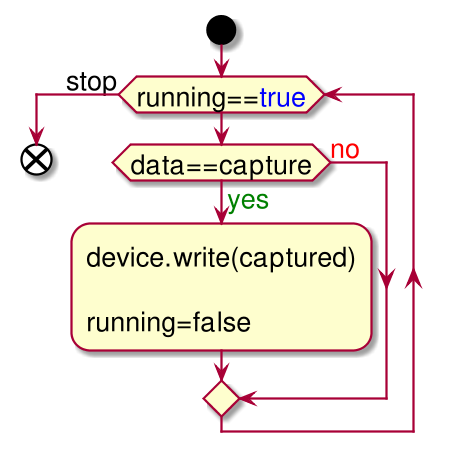
\includegraphics[width=.5\textwidth,keepaspectratio]{imodbuselementwriter_activity}
        \caption[Жизненный цикл компонента \mbwriter]%
            {Жизненный цикл компонента \mbwriter%
                (см. также листинг \ref{lst:tmpl_method_writerimpl})%
            }%
            \label{fig:imodbuselementwriter_activity}
    \end{figure}
\end{center}


Класс \texttt{ModbusElementWriterImpl} реализует паттерн <<Шаблонный метод>>\footnote{Template method} \cite[стр. 309]{book:pattern:band_of_4},
определяя метод слота \texttt{IModbusElement\-Writer::new\-Modbus\-Data()}
и защищенный метод \texttt{IModbus\-Element\-Writer::wri\-te()} --- инвариантные последовательности операций,
определенные виртуальными методами, которые уточняются с помощью наследования \cite[стр. 170]{book:tdd:KentBeck}.

\lstinputlisting[
    language=C++,
    caption=Реализация контракта компонента (см. рисунок \ref{fig:imodbuselementwriter_activity}),
    label=lst:tmpl_method_writerimpl
        ]{Dissertation/listings/cpp/writerimpl_template_method.hpp}


\subsection{Условия изменения состояния}
Как видно из рисунка \ref{fig:modbus_class_uml} проверка условий записи описываются с помощью компонента типа
\mbrelationed --- наследника класса \mbdata.
Этот класс содержит в себе \texttt{value} от родительского класса и правило отношения \texttt{Relation},
отражающих свойство \texttt{relation} из таблицы \ref{tbl:modbus_data_properties}.
При поступлении новых данных по шине Modbus происходит сравнение значений (листинг \ref{lst:comparator:compare}),
согласно выражению \eqref{eq:axiom_modbusdatarelationed}.
\lstinputlisting[
    language=C++,
    caption=Вспомогательный метод для анализа поступающих данных,
    label=lst:comparator:compare
        ]{Dissertation/listings/cpp/comparator.hpp}


Перейдем к более подробному рассмотрению реализаций интерфейса \texttt{IModbusElementWriter} его наследниками,
согласно таблице~\ref{tbl:modbuselement_writer_def}.

\subsubsection{Запись с единичным условием}\label{sec:guard}
Циклограмма функционирования класса \texttt{ModbusGuardedWriter} приведена на рисунке \ref{fig:modbus_guarded_writed}.
Этот класс переопределяет метод родительского класса \texttt{IModbusElementWriter::conditionsMet()}.
\begin{figure}[h!]\begin{center}
    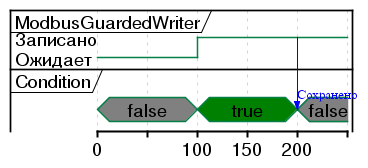
\includegraphics[width=.8\textwidth,keepaspectratio]{modbus_guarded_writer.png}
    \caption[Циклограмма записи значения для единичного условия]
        {Циклограмма записи значения при выполнении условия в момент времени $\tau_1=100$.}
            \label{fig:modbus_guarded_writed}
\end{center}\end{figure}

Как видно из рисунка выполнение условия происходит в момент времени $\tau_1=100$ условных единиц времени,
сразу же по переднему фронту происходит запись нового значения, которое сохраняется даже после окончания
выполнения логического условия \texttt{cond} в $\tau_2=200$.


\subsubsection{Запись со множественными условиями}
Циклограмма функционирования класса \texttt{ModbusMultiguardedWriter} приведена на рисунке \ref{fig:modbus_multiguarded_writed}.
Этот класс переопределяет метод родительского класса \texttt{ModbusElementWriterImpl::newModbusData()},
так как необходимо следить за множеством тегов через этот слот,
заполняется ассоциативный массив (например, \texttt{std::map<std::string, bool>} у которого ключем является
название тега \texttt{modbusio::ModbusElement::title()}, а значением результат выражения
\begin{lstlisting}[language=C++]
    return std::accumulate(list.cbegin(), list.cend(),
        true,
        std::logical_and<>());
\end{lstlisting}
Как видно из рисунка \ref{fig:modbus_multiguarded_writed}, значение не будет записано до тех пор, пока не будут
выполнены все условия, даже если после установления одного из условий оно меняется
(как показано для второго условия на 100 единице времени). Аналогично с \texttt{ModbusGuardedWriter}
после того как значение было записано, выполнение условий не контролируется, 
при этом записанное значение сохраняется, но может быть независимо изменено по другим причинам,
так как компонент больше не владеет ресурсом и отписывается от событий.
\begin{figure}[h!]\begin{center}
    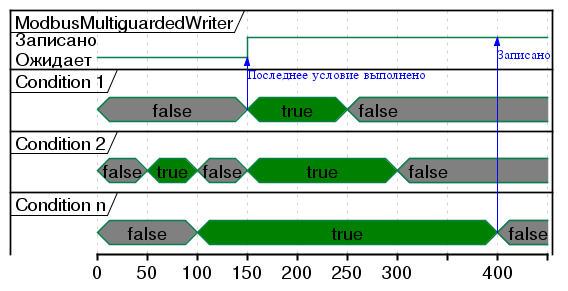
\includegraphics[width=.8\textwidth,keepaspectratio]{modbus_multiguarded_writer.png}
    \caption{Циклограмма записи значения при выполнении множественных условий.}
        \label{fig:modbus_multiguarded_writed}
\end{center}\end{figure}



\subsubsection{Отложенная запись с единичным условием}
Циклограмма функционирования класса \texttt{ModbusDelayedWriter} приведена на рисунке \ref{fig:modbus_delayed_writer}.
Этот класс уточняет метод родительского класса \texttt{ModbusGuardedWriter::conditionsMet()},
при выполнении условия которого запускается таймер на время задержки \texttt{delay},
по окончании которого происходит запись значения.
% \begin{center}
%     \begin{figure}[h!]
%         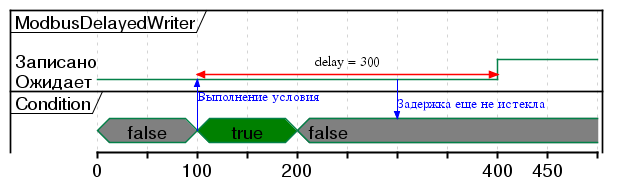
\includegraphics[width=.8\textwidth,keepaspectratio]{modbus_delayed_writer.png}
%         \caption{Циклограмма отложенной записи значения при выполнении единственного условия.}\label{fig:modbus_delayed_writer}
%     \end{figure}
% \end{center}
Класс позволяет устанавливать значение после выполнения условия и по истечению задержки $\tau$.
По окончании таймера на запись значение выражения \texttt{Condition} не анализируется
и запись происходит в любом случае.


\subsubsection{Отложенная запись со множеством условий}
Циклограмма функционирования класса \texttt{ModbusDelayedMultiguardWriter} приведена на рисунке \ref{fig:modbus_delayed_multiguarded_writer}.
Этот компонент переопределяет метод \texttt{IModbusElementWriter::newModbusData()},
а запуск таймера осуществляется при достижении истинного значения
функции супер-класса \texttt{ModbusMultiguardedWriter::conditionsMet()}.

\subsubsection{Периодическая запись}
Данный компонент предназначен для реализации периодических событий, как показано на диаграмме \ref{fig:modbus_periodic_writer}.
При захвате управления дискретной переменной, ее значение инвертируется каждый период
$f_i(x; \tau) = \lnot f_{i-1}(x; \tau)$, причем $f(x; \tau) \in \{0, 1\}$
(на графике сверху захвачен булевский тег, период равен 25 единиц времени, длительность не ограничена).
При захвате вещественной переменной значение меняется по закону
$f_i(x,\Delta x; \tau) = f_{i-1}(x,\Delta x; \tau) + \Delta x, \Delta x \in \mathcal{R}$
(на графике снизу период равен 50 единиц времени, $\Delta x = 10$ на 200 единиц времени).

Этот компонент используется, например, для управления значениями количества оборотов,
количества транзакций и пакетов, переданных от контроллера к программе верхнего уровня,
при захвате вещественных переменной (как уже обсуждалось в разделе \ref{sec:model_anpa_params}).
Очевидно, что приращение $\Delta x$ может быть как положительным, так и отрицательным.

Если в конфигурации сценария (листинг \ref{lst:modbus_periodic_writer_xml}) имеется атрибут
\texttt{duration}, компонент будет работать от выполнения условий до окончания указанной длительности.
В противном случае обновление значений будет происходить до момента прекращения работы
путем вызова функции \texttt{IModbusElementWriter::reset()}.

\begin{figure}[h!]\begin{center}
    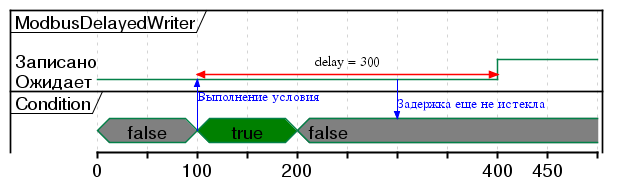
\includegraphics[width=.8\textwidth,keepaspectratio]{modbus_delayed_writer.png}
    \caption{Циклограмма отложенной записи значения при выполнении единственного условия.}\label{fig:modbus_delayed_writer}
    %
    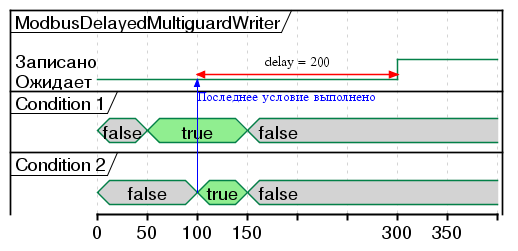
\includegraphics[width=.8\textwidth,keepaspectratio]{modbus_delayed_multiguarded_writer.png}
    \caption{Циклограмма отложенной записи значения при выполнении множественных условий.}\label{fig:modbus_delayed_multiguarded_writer}
    %
    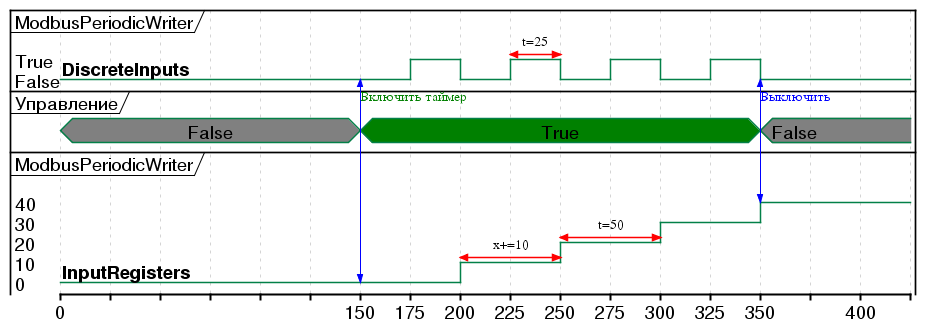
\includegraphics[width=.8\textwidth,keepaspectratio]{modbus_periodic_writer.png}
    \caption{Циклограмма периодической записи значения.}\label{fig:modbus_periodic_writer}
\end{center}\end{figure}



\subsection{Реализация интерфейса \mbdevice}
Для реализации интерфейса \mbdevice также используется возможность множественного наследование языка программирования \cpp:
одним из родителей является интерфейс \mbdevice,
а вторым --- класс библиотеки~\texttt{Qt}, обеспечивающий реализацию физической передачи информации по протоколу Modbus
\texttt{QModbusTcpServer}, так как обмен происходит по разновидности протокола Modbus TCP/IP.
Упрощенная реализация показана в листинге~\ref{lst:imodbus_device_impl}.
\begin{figure}[hb!]\begin{center}
        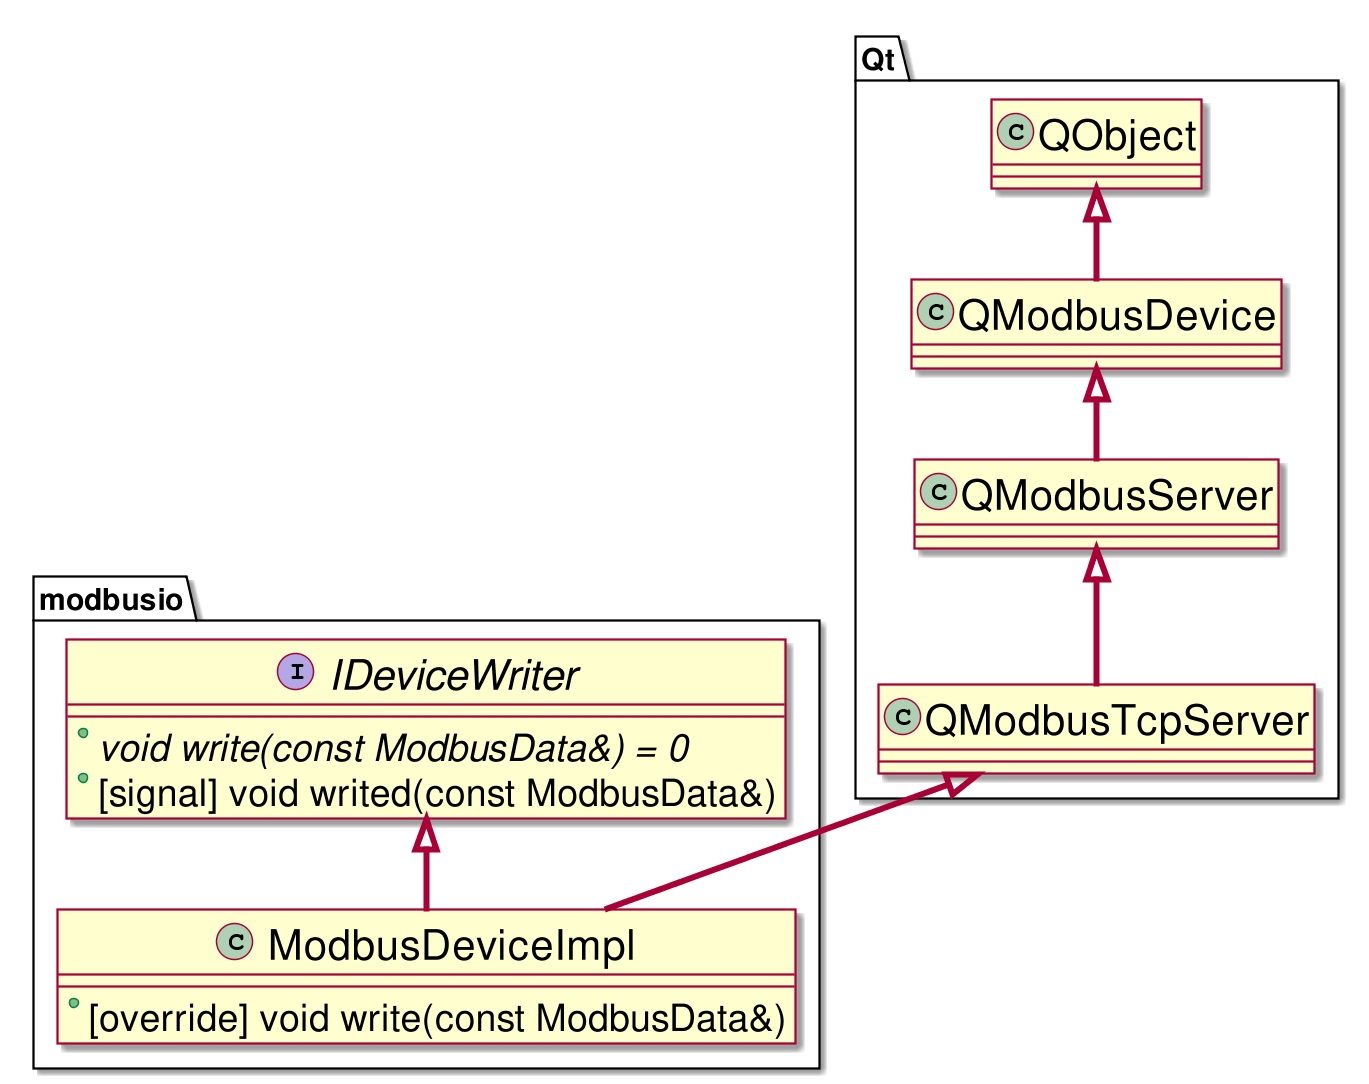
\includegraphics[width=.6\textwidth,keepaspectratio]{modbus_device_impl.png}
        \caption[Реализация интерфейса устройства записи.]
            {Реализация устройства для записи значений по протоколу Modbus}\label{fig:modbus_device_imp}
\end{center}\end{figure}
\lstinputlisting[
    language=C++,
    caption=Простейшая реализация \mbdevice устройства,
    label=lst:imodbus_device_impl]
        {Dissertation/listings/cpp/dummydeviceimpl.hpp}
Таким образом используется интерфейс вместо конкретной реализации \cite[стр. 47-48]{book:pattern:head_first}


\subsection{Описание конфигурационного файла для компонентов интерфейса \mbwriter}
Каждая группа должна быть помещена в корневой элемент \texttt{Scenario},
как показано в листинге \ref{lst:modbus_scenario_example_diagram} приложения \ref{app:sec:modbus_scenario_example_diagram}.

Каждый компонент помещается внутри тега \texttt{Writer} (представляющий класс всех возможных изменений $\mathbb{A}$, см. раздел \ref{sec:ontology}),
с обязательным текстовым атрибутом \texttt{tag}, который указывает каким ресурсом владеет данный компонент
и обязательным атрибутом \texttt{value} (см. листинг \ref{lst:modbus_tags_scenario_configs}).
Также есть ряд необязательных атрибутов, о которых будет сказано отдельно. 
Одновременно владеть одним и тем же ресурсом могут несколько компонентов (как будет показано ниже).
Далее следует секция условий --- \texttt{Conditions},
описывающая классы отношений $\mathbb{C}$ (см. также выражение \eqref{eq:axiom_modbusdatarelationed}).
Каждое условие описывается логической операцией отношения \texttt{relation} для смежного параметра,
указанного в обязательном поле \texttt{tag} и связанного с ним значения \texttt{value}.
Элемент \texttt{relation} принимает одно из следующих значений:
\texttt{eq} ($=$),
\texttt{ne} ($\neq$),
\texttt{gt} ($>$),
\texttt{lt} ($<$),
\texttt{ge} ($\geq$),
\texttt{le} ($\leq$), по аналогии с обозначениями в языке Fortran.
Отношение типа \texttt{eq} считается отношением по умолчанию,
все остальные отношения же необходимо указывать явным образом.
Необязательным полем является поле \texttt{Purpose}, в котором размещается информация для
обозначения назначения компонента в сценарии.

\subsubsection{ModbusGuardedWriter}
Рассмотрим более подробно описание компонента для записи с единичным условием,
который размещается в элементе \texttt{Guarded} листинга~\ref{lst:modbus_guarded_writer_xml}:
\lstinputlisting[
    language=MyXML,
    caption=Пример конфигурации \texttt{ModbusGuardedWriter},
    label=lst:modbus_guarded_writer_xml]
        {Dissertation/listings/xml/guarded.xml}
Захватывается управление над тегом \texttt{A1}, которой будет присвоено значение 160
при выполнении условия \texttt{R1 = true}.
Иными словами при истинности предиката $P$ будет выполнено действие $Q$:
$P(R1=\mbox{true}) \to Q(A1=160)$.


\subsubsection{ModbusMultiguardedWriter}
Для описания компонента со множественными условиями, используется следующий формат,
который размещается в элементе \texttt{Multiguarded} листинга~\ref{lst:modbus_multiguarded_writer_xml}:
\lstinputlisting[
    language=MyXML,
    caption=Пример конфигурации \texttt{ModbusMultiguardedWriter},
    label=lst:modbus_multiguarded_writer_xml]
        {Dissertation/listings/xml/multiguarded.xml}
Переменной \texttt{Regime} будет присвоено значение 1, как только 
одновременно будет выполнено два условия: $Regime = 1: \{A1 \ge 150 \wedge C1 = true\}$.
Таким образом $P(x_1,\ldots,x_n) = P(A1\ge150, C1=\mbox{true}) \to Q(Regime=1)$.

\subsubsection{ModbusDelayedWriter и ModbusDelayedMultiguardWriter}
Компоненты этого типа располагаются в окружении тегов элементов \texttt{Delayed} и \texttt{Multidelayed}, соответственно,
как показано в листинге~\ref{lst:modbus_delayed_writer_xml}.
\lstinputlisting[
    language=MyXML,
    caption=Пример конфигурации \texttt{ModbusDelayedWriter} и \texttt{ModbusDelayedMultiguardWriter},
    label=lst:modbus_delayed_writer_xml]
        {Dissertation/listings/xml/delayed.xml}
Очевидно, что происходит захват управления значения переменной \texttt{PP\_1}, которой будет установлено значение \texttt{true}
через 50 единиц времени, как только будут выполнены два условия:
$PP\_1 = \mbox{true}: \{R1 = \mbox{true} \wedge A1 \le 150\}$.
Или используя предикатные обозначения
$P(x_1,\ldots,x_n) = P(A1\le150, R1=\mbox{true}, \tau=50) \to Q(PP\_1=\mbox{true})$.


\subsubsection{ModbusPeriodicWriter}
Данный компонент располагается внутри элемента \texttt{Period} в конфигурационном файле сценария,
согласно листингу~\ref{lst:modbus_periodic_writer_xml}.
\lstinputlisting[
    language=MyXML,
    caption=Пример конфигурации \texttt{ModbusPeriodicWriter},
    label=lst:modbus_periodic_writer_xml]
        {Dissertation/listings/xml/periodic.xml}
В данном примере дистанция, ассоциированная с переменной \texttt{Distance}, увеличивается на 100 единиц каждые 1000 единиц времени,
при выполнении ряда условий, а именно: $\{C1 = true \wedge A1 > 100 \wedge A1 \le 150 \}$ или
увеличивается на теже 100 единиц, но с периодом 500 единиц, когда достигаются следующие условия:
$\{C1 = true \wedge A1 > 150\}$
Отметим, что для этого компонента начальное значение устанавливается с помощью атрибута \texttt{value}
при вызове метода \texttt{IModbusElementWriter::start()}.


\subsection{Сводная таблица наследников \texttt{IModbusElementWriter}}
Общая информация о компонентах представлена в таблице~\ref{tbl:ModbusElementWriterImpl}.
Из этой таблицы видно, что использование наследования совместно с паттерном <<шаблонный метод>>
позволяет переопределять поведение компонентов, обеспечивая выполнение контрактов наследниками интерфейса
\cite[стр. 124-125]{book:oop:oop_analize,bib:my:ttd_with_patterns_2019}.

\begin{table}[h!]
\begin{center}
\caption{Сводная таблица \textit{метаклассов} модели АНПА.}\label{tbl:ModbusElementWriterImpl}
\begin{tabular}{|l|c|c|c|c|c|c||c|c|}
\hline
    \multicolumn{1}{|c|}{\multirow{2}{*}{Наследники}} &
    \multicolumn{6}{c||}{\textbf{атрибуты}} &
    \multicolumn{2}{c|}{\textbf{override}} \\ \cline{2-9} %Переопределенные методы наследника
    \multicolumn{1}{|c|}{}     &
        \rotatebox{90}{tag} & \rotatebox{90}{value}  & \rotatebox{90}{delay}  & \rotatebox{90}{period} &
        \rotatebox{90}{delta} & \rotatebox{90}{duration} &
        \rotatebox{90}{conditionsMet} & \rotatebox{90}{newModbusData} \\ \hline
    \texttt{ModbusGuardedWriter}              & +    & +      & -      & -      & - &-     & + & -  \\ \hline
    \texttt{ModbusMultiguardedWriter}         & +    & +      & -      & -      & - &-     & + & -  \\ \hline
    \texttt{ModbusDelayedWriter}              & +    & +      & +      & -      & - &-     & - & +  \\ \hline
    \texttt{ModbusDelayedMultiguardWriter}    & +    & +      & +      & -      & - &-     & - & +  \\ \hline
    \texttt{ModbusPeriodicWriter}             & +    & +      & -      & +      & + &$\pm$ & + & -  \\ \hline
\end{tabular}
\end{center}
\end{table}


\section{Менеджер индивидов класса \mbwriter имитатора}
Для управления компонентами имитатора используется менеджер компонентов \texttt{ModbusIoManager}.
Установка компонентов производится с помощью экземпляра класса \texttt{ScenarioParser}, реализующего интерфейс \texttt{IParser}.
Этот интерфейс является общим как для чтения файла сценария (листинг~\ref{lst:modbus_scenario_example_diagram}),
так и для файла тегов (листинг \ref{lst:modbus_tags_example}).
При чтении конфигурации проверяется, что каждый тег $t_i$ типа \mbdata,
управление над которым захватывается, или условия выполнения переходов типа \mbrelationed,
являются элементами множества класса первичных данных, то есть $\forall t_i \in \mathbb{T}$ (см. раздел \ref{sec:ontology}).

На рисунке \ref{fig:modbus_class_components} показано отношение между менеджером \texttt{ModbusIoManager},
интерфейсом парсера \texttt{IParser} и интерфейсом \mbwriter.
\begin{center}
    \begin{figure}[hb!]
        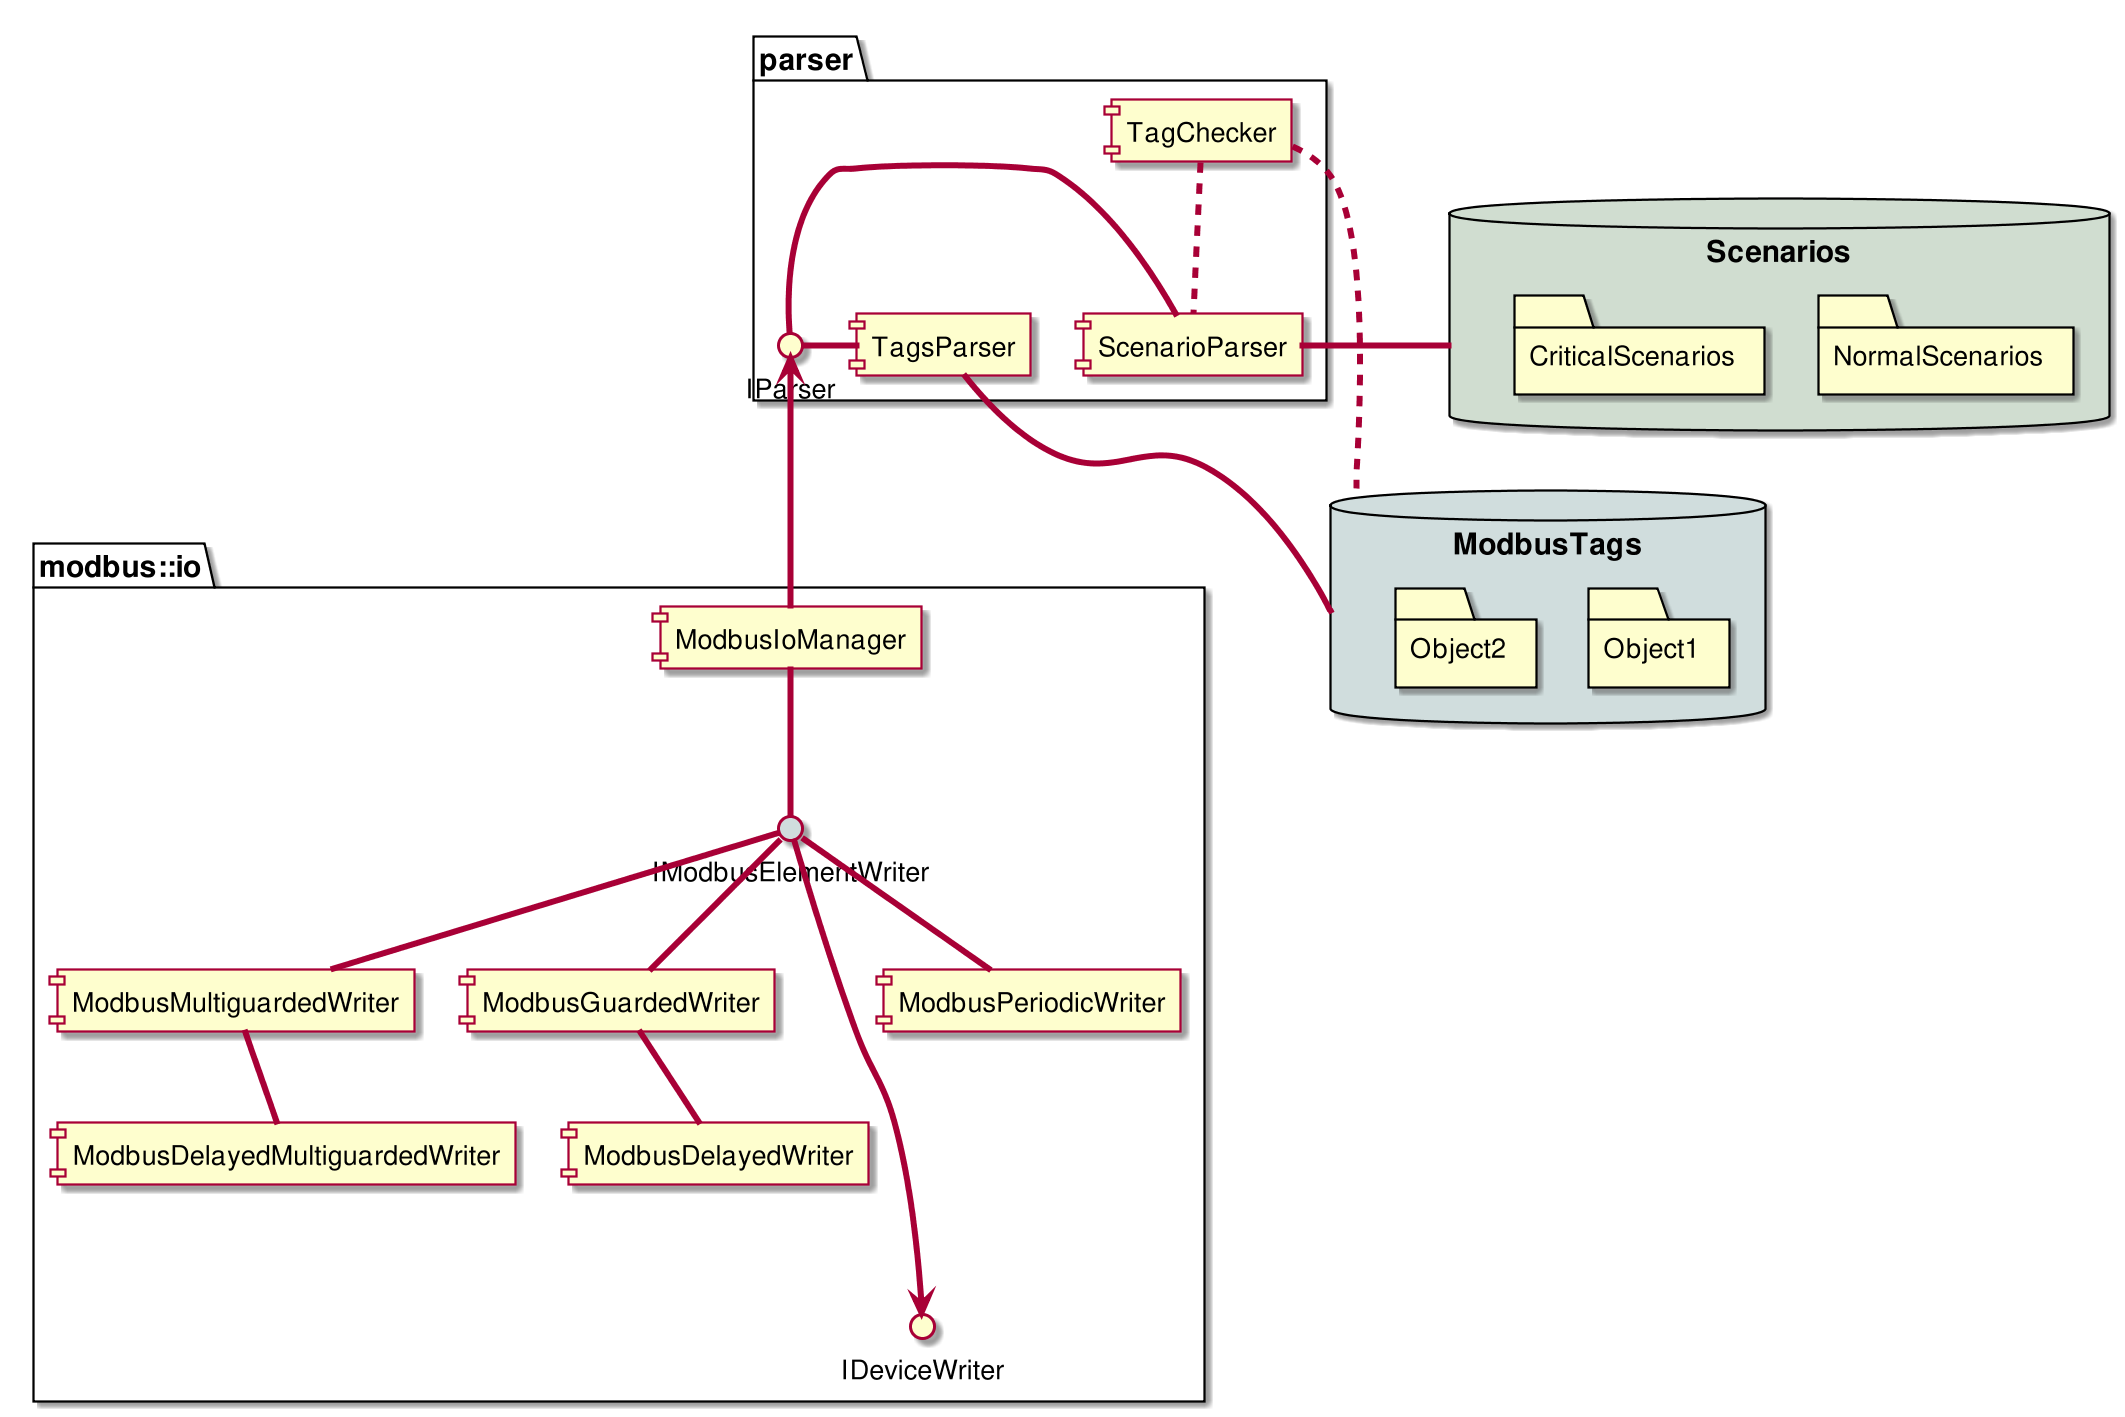
\includegraphics[width=.9\textwidth,keepaspectratio]{modbus_class_components}
        \caption{Композиция классов менеджера сценариев.}\label{fig:modbus_class_components}
    \end{figure}
\end{center}


Последовательность действий по конфигурированию окружения программного обеспечения
показана на рисунке~\ref{fig:top_level_sequence} \cite[стр. 239]{book:oop:oop_analize}.
\begin{center}
    \begin{figure}
        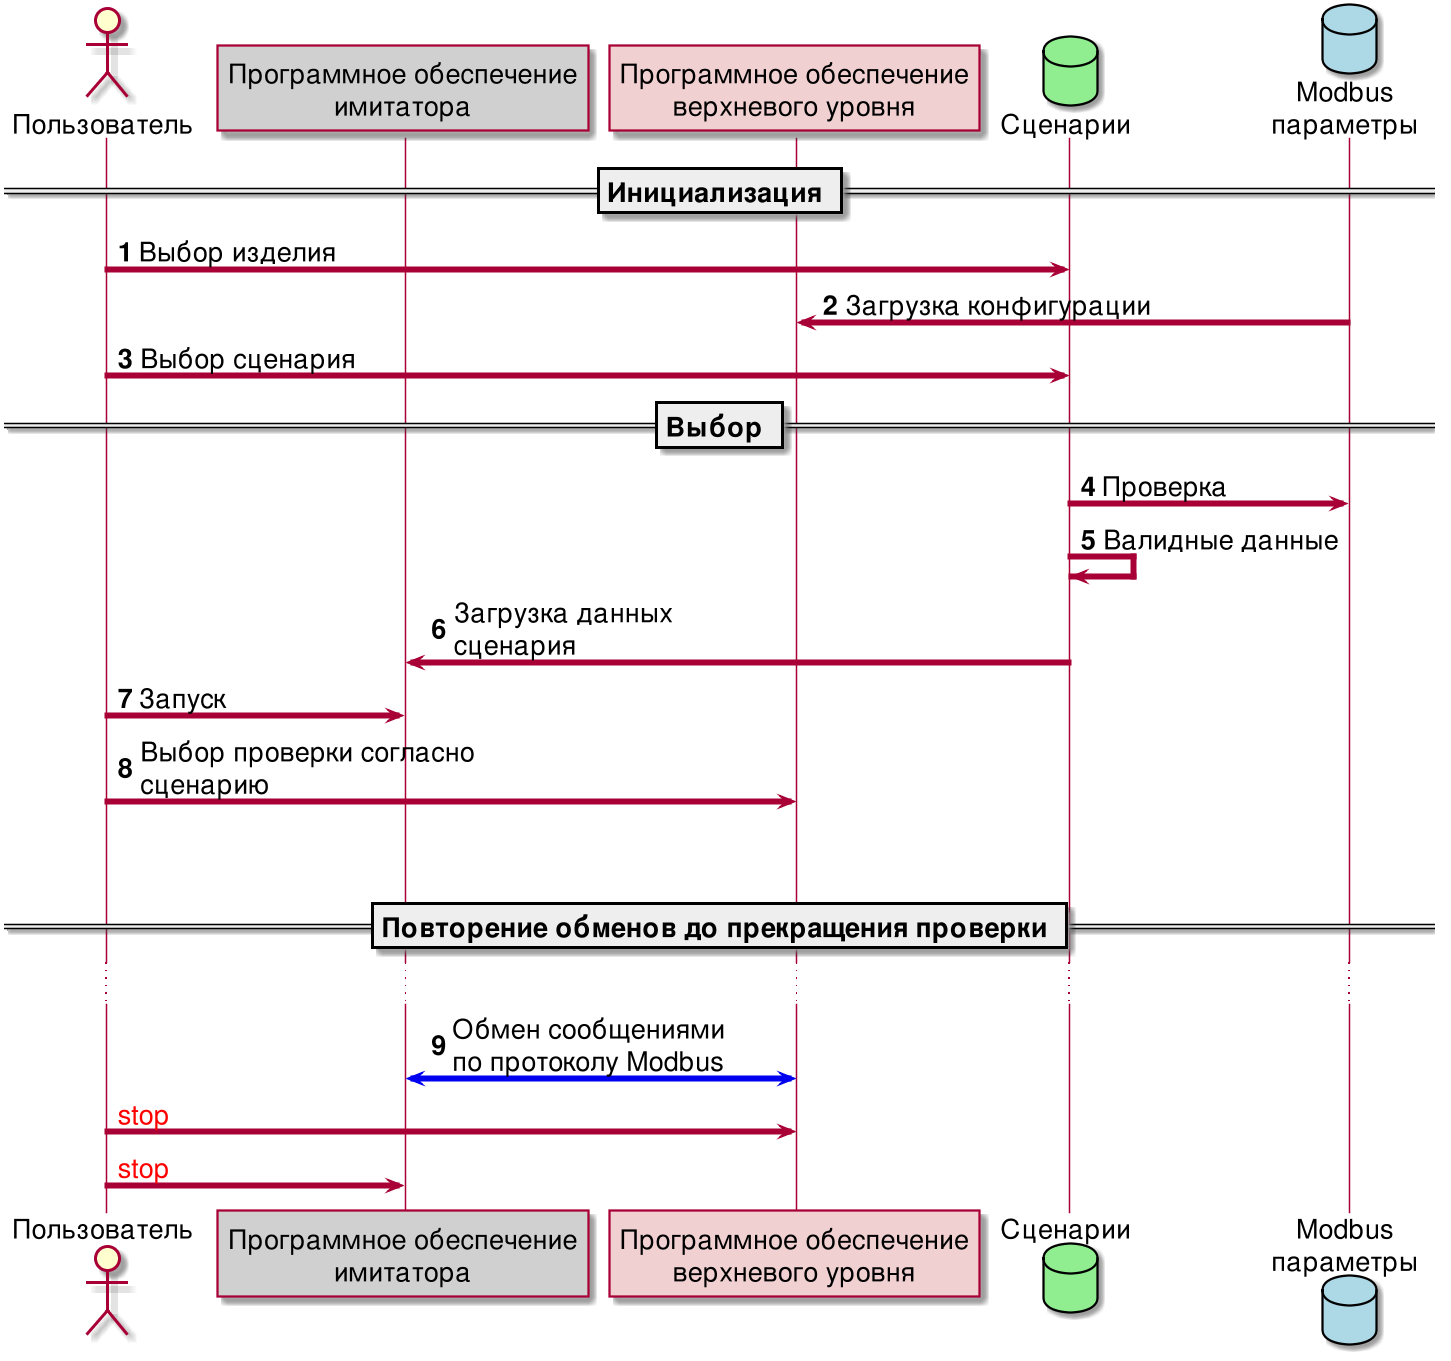
\includegraphics[width=.9\textwidth,keepaspectratio]{top_level.png}
        \caption{Последовательность действий при работе с имитатором}
        \label{fig:top_level_sequence}
    \end{figure}
\end{center}

\textbf{Инициализация и загрузка конфигурации.}
На этом этапе происходит настройка программного обеспечения
имитатора и программы, так называемого, верхнего уровня,
то есть программного обеспечения непосредственно системы контроля.
В случае корректной конфигурации происходит запуск
выбранной проверки оператором.

\textbf{Выполнение сценария проверки.}
После запуска две программы начинают обмениваться 
сообщениями по протоколу Modbus~TCP/IP, например внутри локальной сети.
Более подробно этот этап показан на рисунке \ref{fig:modbuselementwriterimpl}.

\textbf{Окончание проверки.}
Происходит возврат к исходным настройкам систем и отключение.
После этого процедура может быть воспроизведена вновь с теми же
или другими параметрами. 

\begin{center}
    \begin{figure}
        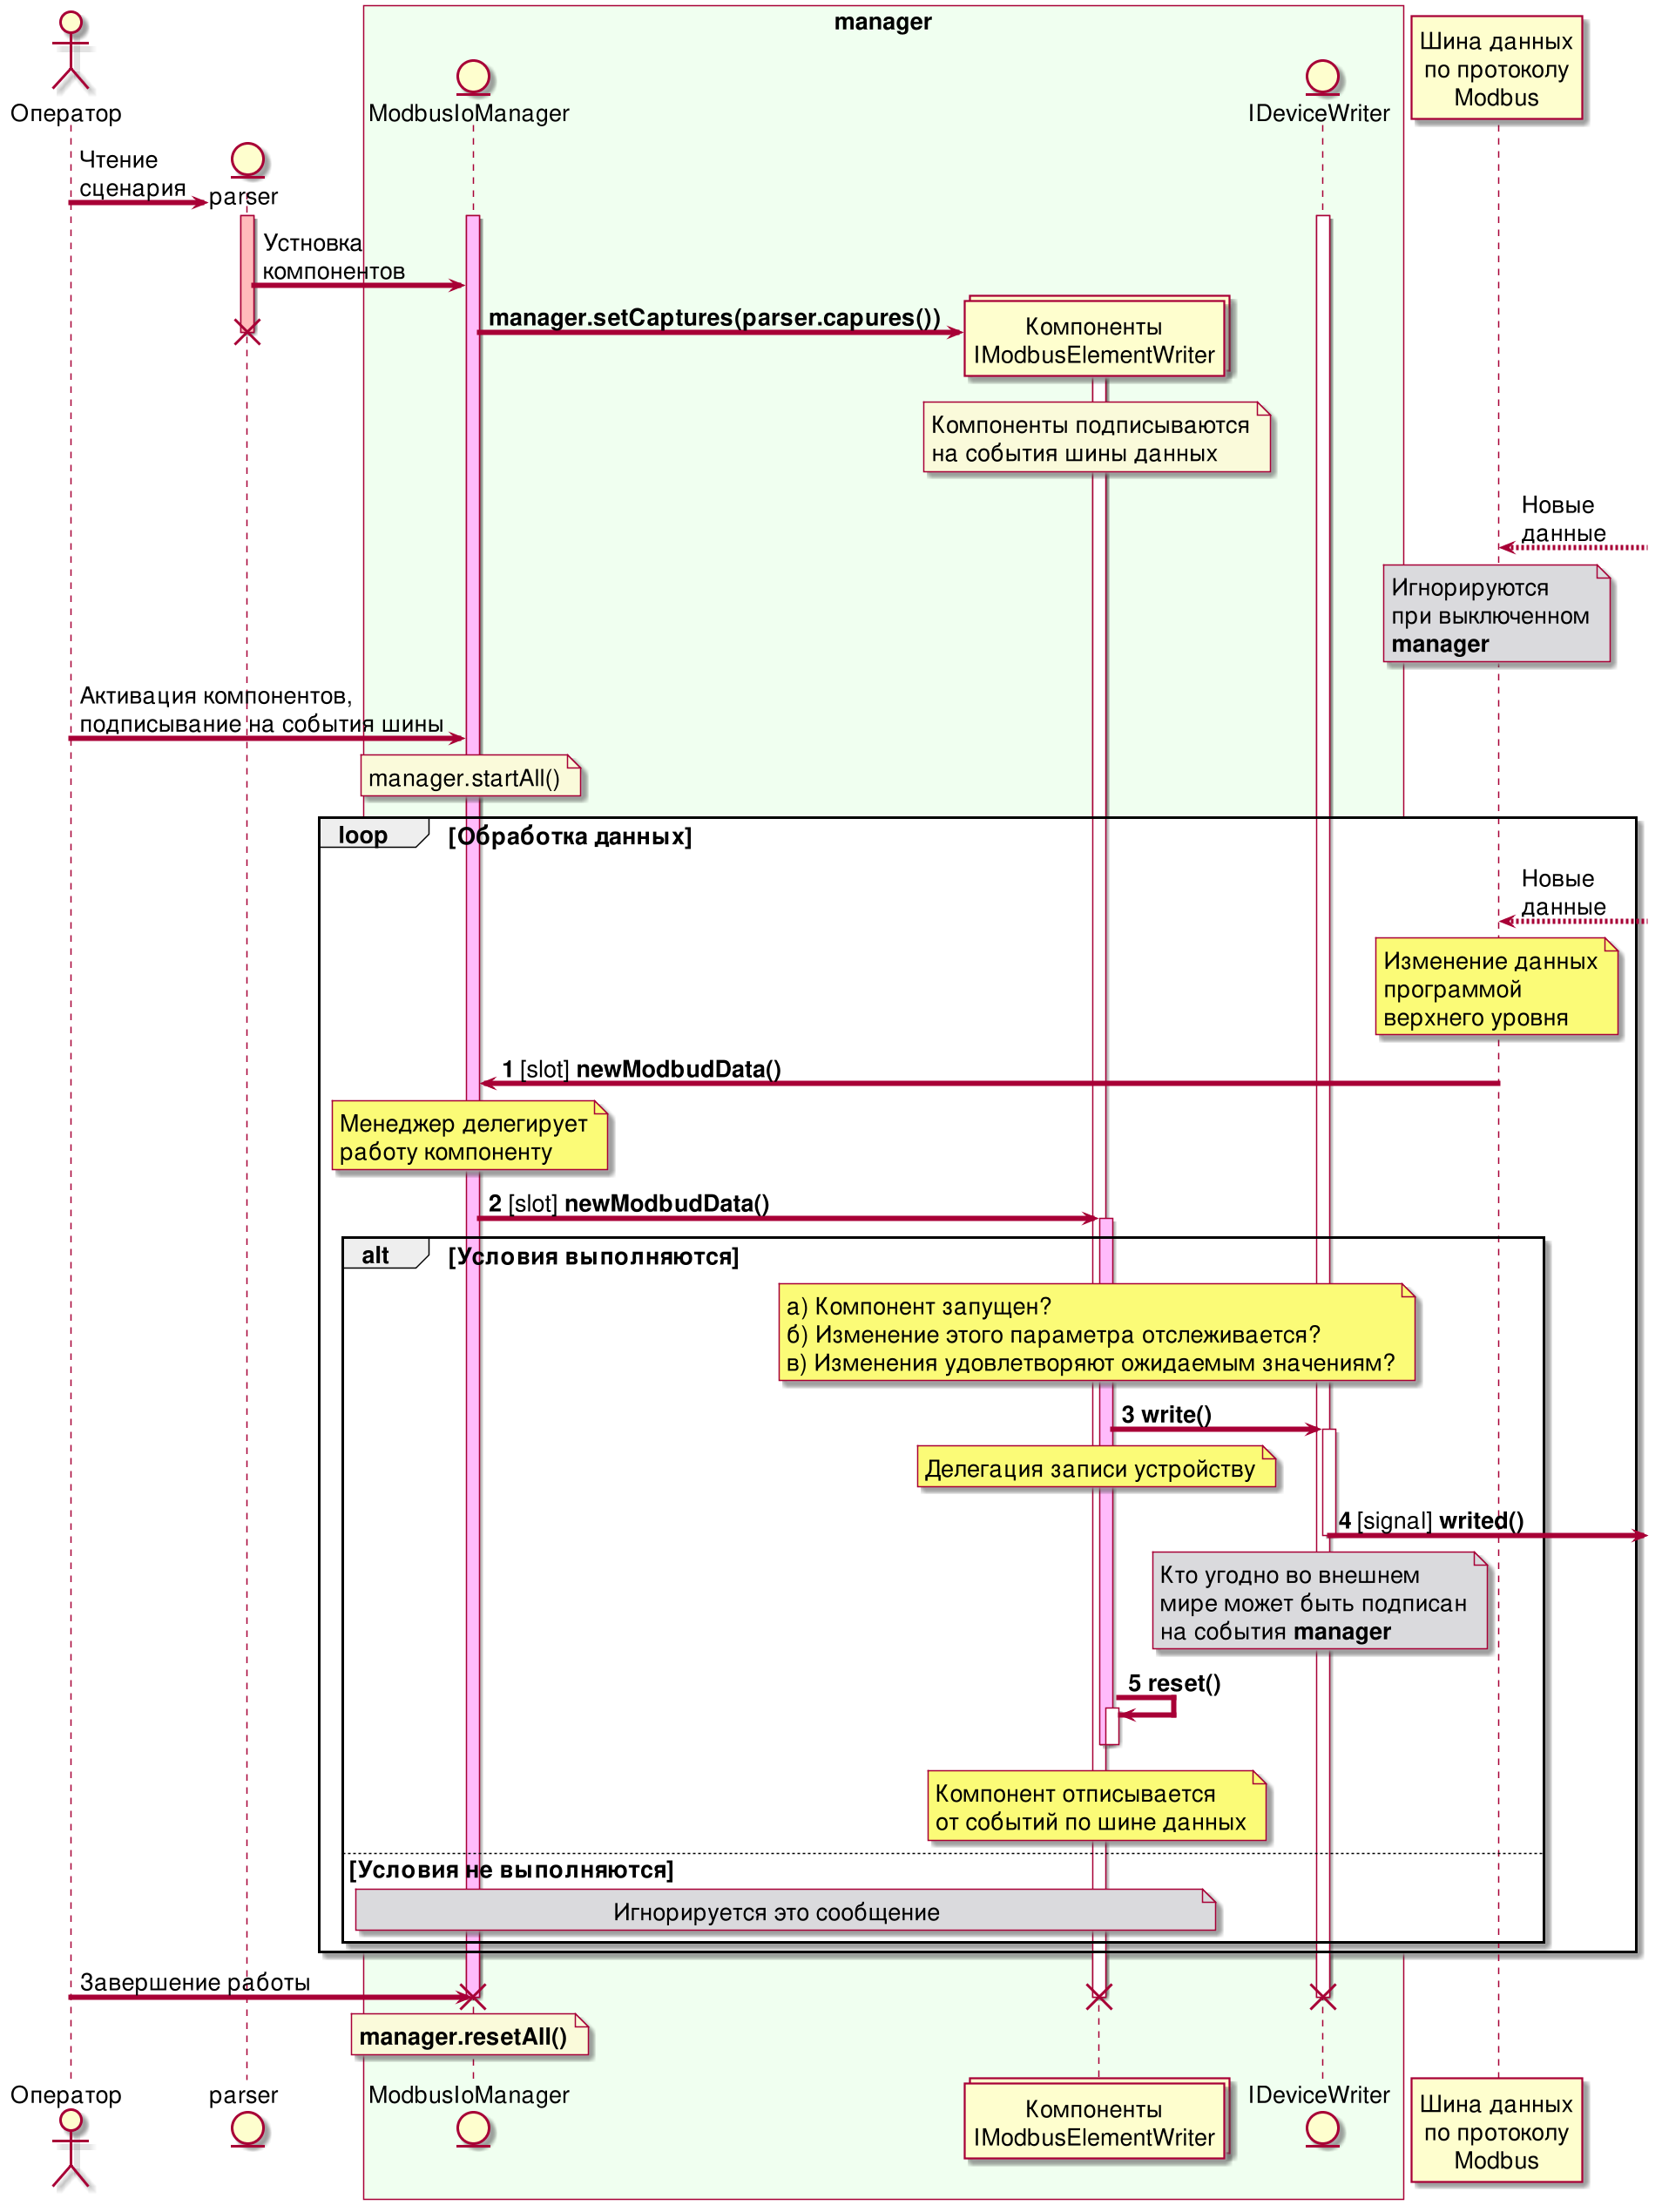
\includegraphics[height=.8\textheight,keepaspectratio]{modbuselementwriterimpl.png}
        \caption[Взаимодействие компонентов с шиной данных]
            {Взаимодействие компонентов с шиной данных (см. также листинг \ref{lst:tmpl_method_writerimpl})}
        \label{fig:modbuselementwriterimpl}
    \end{figure}
\end{center}


\textbf{Обработка данных при выполнении сценария проверки.}
Как было сказано ранее, после запуска менеджера \texttt{modbusio::\-ModbusIoManager::\-start\-All()}
менеджер готов к обработке данных.
До этого момента приходящие сообщения игнорируются им.

Таким образом, менеджер подписывается на изменения данных по шине Modbus,
через слот \texttt{newModbusData()}.
Работа с поступающими данными делегируется экземплярам, реализующих интерфейс
\mbwriter, после чего происходит проверка поступающих данных по следующим пунктам.
\begin{enumerate}
    \item Запущен ли компонент.
    \item Изменение это параметра отслеживается. Как было сказано ранее в разделе \ref{sec:ontology}
        два и более компонентов могут быть изоморфны относительно входного сигнала,
        таким образом, очевидно что этот сигнал перенаправляется всем компонентам,
        которыми владеет менеджер.
    \item Происходит проверка все ли предикаты в правилах перехода в значении истина. 
\end{enumerate}
При выполнении всех трех пунктов хотя бы для одного компонента,
происходит запись значения $P(x_1, \ldots, x_n) \to Q(x)$.
Компонент делегирует это экземпляру, реализующему интерфейс \mbdevice,
через вызов виртуальной функции \texttt{IDeviceWriter::write()}.
В следствии этого компонент отписывается от событий по шине данных,
вызовом функции \texttt{IModbusElementWriter::reset()}.

Обработка данных при выполнении сценария проверки происходит до тех пор
пока менеджер не будет остановлен \texttt{ModbusIoManager::resetAll()}.


\section{Пример композиции для простейшего сценария}

Рассмотрим пример сценария на основе множества Modbus тегов из листинга \ref{lst:modbus_tags_example},
циклограмма которого представлена на рисунке \ref{fig:modbus_scenario_example_diagram},
сценарий приведен в листинге \ref{lst:modbus_scenario_example_diagram} в разделе приложения \ref{app:sec:modbus_scenario_example_diagram}.
Схема разметки приведена в листинге \ref{lst:modbus_tags_scenario_configs}.

\begin{landscape}
    \begin{center}
        \begin{figure}
            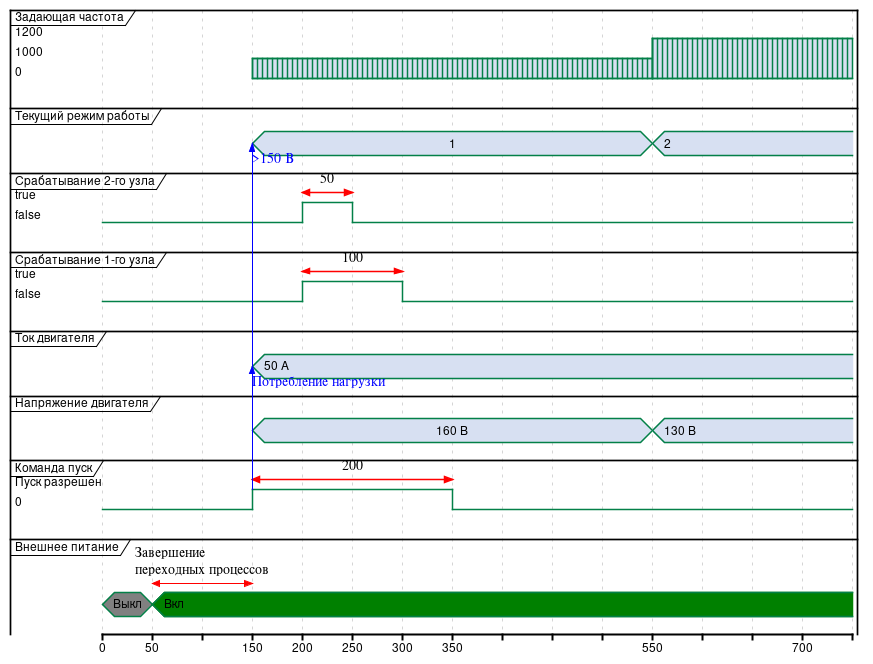
\includegraphics[height=.8\textheight,keepaspectratio]{modbus_scenario_example_diagram.png}
            \caption{Пример использования классов.}\label{fig:modbus_scenario_example_diagram}
        \end{figure}
    \end{center}
\end{landscape}


\section*{Заключение}
Продемонстрирован унифицированный способ представления субъектно-ориентированного механизма
изменения параметров, для имитации как внешнего так и внутреннего окружения объекта контроля.
Создана онтологическая модель автономного необитаемого подводного аппарата.
На основе проведенных исследований модели создана программная реализация 
с использованием языка программирования \cpp и библиотки \texttt{Qt}.
